\documentclass[12pt,oneside,a4paper,notitlepage]{report}

\usepackage[backend=biber,sorting=none,maxbibnames=99]{biblatex}
\usepackage{setspace}
\usepackage{graphicx}
\usepackage{syntax}
%\usepackage{wasysym}
\usepackage{textcomp}
\usepackage{newfloat}

\title{
	Implementing an Object Model for TDL\textsuperscript{TP} Expressions
}
\author{Tanel Prikk}

\DeclareFloatingEnvironment[
fileext   = logr,
listname  = {List of Grammars},
name      = Grammar,
placement = htp
]{GrammarWrapper}
\setlength{\grammarindent}{5em}
\setlength{\grammarparsep}{5pt plus 1pt minus 1pt}

\newcommand{\texttilde}{\raisebox{0.5ex}{\texttildelow}}

\addbibresource{Sources.bib}
\pagenumbering{gobble}
\singlespacing


\begin{document}
	\maketitle

	\section*{Background}
	\par Our ANTLR-generated parser is capable of building parse trees for TDL\textsuperscript{TP} expressions. The object structure of said trees is, however, dependent on the ANTLR library. Higher-level components that will work with TDL parse trees should be decoupled from this implementation detail. To achieve this, we define an independent object model which provides facilities for storage and manipulation of TDL parse trees. In the future, we will also write an adapter for converting ANTLR TDL parse trees to objects from our independent object model.

	\newpage

	\section*{Requirements Analysis}
	\par Considering that in we need to work with a parse tree (concrete syntax tree), a suitable data structure for storing this is a rooted ordered tree. A classical implementation of such a tree is pointer-based. We provide a class diagram below:

	\begin{figure}[h]
		\begin{center}
		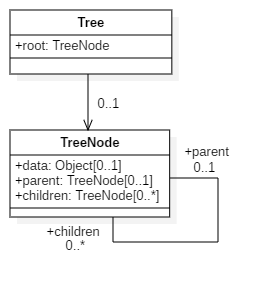
\includegraphics{Models/BasicTree}
		\end{center}
		\caption{Tree class diagram.}
		\label{fig:basic-tree}
	\end{figure}

	\par A simple approach would directly utilize the tree data structure from figure~\ref{fig:basic-tree} and provide implementations only for the data objects that will be referenced in \texttt{TreeNode} instances. However, this is too inconvenient to work with as consumers of the object model would have to be aware of the syntax rules for TDL in order to use the parse tree effectively. A better approach is to provide specific \texttt{TreeNode} implementations per expression type. This allows us to encode structural rules in the APIs of parse tree nodes.

	\newpage

	\par To begin specifying \texttt{TreeNode} sub-classes, we should take into consideration the grammar for the language, reproduced below:

	\begin{GrammarWrapper}
		\begin{grammar}
			% https://tex.stackexchange.com/questions/24886/which-package-can-be-used-to-write-bnf-grammars
			% http://texdoc.net/texmf-dist/doc/latex/mdwtools/syntax.pdf
			<Expression>	::=	'(' <Expression> ')'
			\alt 				'A' '(' <TrapsetExpression> ')'
			\alt 				'E' '(' <TrapsetExpression> ')'
			\alt 				<UnaryOp> <Expression>
			\alt 				<Expression> <BinaryOp> <Expression>
			\alt 				<Expression> '\texttilde' '\textgreater' <Expression> 
			\alt 				<Expression> '\texttilde' '\textgreater' '[' <RelOp> <NUM> ']' <Expression> 
			\alt 				'\#' <Expression> '[' <RelOp> <NUM> ']'
			
			<TrapsetExpression>	::=	'(' <TrapsetExpression> ')'
			\alt						'!' <ID>
			\alt 						<ID> '\textbackslash' <ID>
			\alt						<ID> ';' <ID>
			
			<UnaryOp>	::= '\texttilde'
			
			<BinaryOp>	::= '\&' | '|' | '-' '\textgreater' | '\textless' '-' '\textgreater'
			
			<RelOp> 	::= '\textless' | '=' | '\textgreater' | '\textless' '=' | '\textgreater' '='
			
			<ID> 		::= 'TR' <NUM>
			
			<NUM> 		::= ('0' ... '9')+
		\end{grammar}
		\caption{TDL\textsuperscript{TP} grammar}\label{bnf:modified}
	\end{GrammarWrapper}

	\newpage

	\par Based on grammar~\ref{bnf:modified}, we can produce the following broad classification for nodes in a TDL expression parse tree:

	\begin{table}[h]
		\caption{Parse tree node types}
		\centering
		\makebox[\textwidth]{
			\begin{tabular}{l l l}
				\hline
				Node type & Maximum arity & Child nodes \\
				\hline
				Logical expression & quaternary & l. operator, l. expressions, bound, q. trapset expressions \\
				Bound & binary & bound operator, natural number \\
				Quantified trapset expression & binary & quantifier, trapset expression \\
				Trapset expression & ternary & trapset operator, trapset symbols \\
				Trapset symbol & N/A & N/A \\
			\end{tabular}
		}
		\label{tbl:parse-tree-node-types}
	\end{table}

	\par Note the following:
	\begin{itemize}
		\item the root node is a logical expression node;
		\item only trapset symbol nodes do not have an operator;
		\item only logical expression nodes can have children of the same type;
		\item only logical expression nodes and quantified trapset expression nodes can be negated.
	\end{itemize}

	Let's define 4 subclasses. 

	\section*{Implementation}
	\par Stub.

	\subsection*{Technology}
	\par Stub.

	\subsection*{Technical Details}
	\par Stub.

	\printbibliography[
		title=Sources
	]

\end{document}
